\section{Methodology}
\label{sec:5_methods}

% ==================== Model Selection and Justification ==================== %
\subsection{Model Selection and Justification}
\label{sec:model_selection_and_justification}
This thesis employ two probabilistic deep learning architectures: LSTM-Mixture Density Network (LSTM-MDN) and Transformer-Mixture Density Network (Transformer-MDN). The models are selected due to their ability to capture complex, non-linear dependencies in financial time series while providing full conditional probability distributions. Unlike traditional econometric models that rely on restrictive parametric distributions—such as Gaussian or Student-t distributions—these proposed probabilistic AI models allows for a flexible non-parametric conditional distributional forecasts. Model architecture overview for the two models are illustrated in Figure \ref{fig:model_architectures}.

\begin{figure}[H]
    \centering
    \begin{subfigure}[b]{0.49\textwidth}
        \centering
        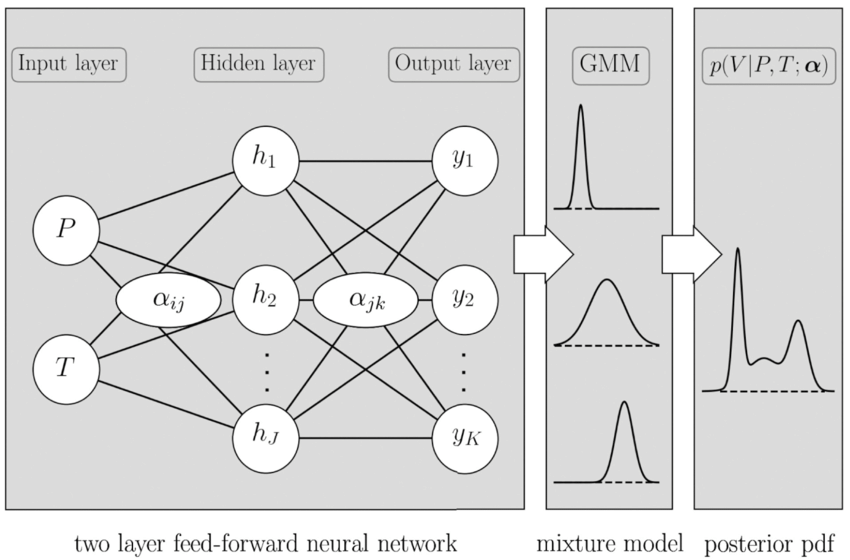
\includegraphics[width=\linewidth, height=5cm]{Images/Methods/model_architecture_LSTM_MDN.png}
        \caption{Architecture of the LSTM-MDN model, combining a Long Short-Term Memory network with a Mixture Density Network.}
        \label{fig:model_architecture_LSTM_MDN}
    \end{subfigure}
    \hfill
    \begin{subfigure}[b]{0.49\textwidth}
        \centering
        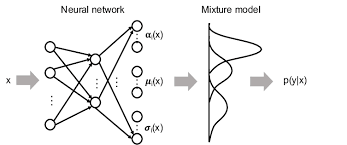
\includegraphics[width=\linewidth, height=5cm]{Images/Methods/model_architecture_Transformer_MDN.png}
        \caption{Architecture of the Transformer-MDN model, integrating a Transformer encoder with a Mixture Density Network.}
        \label{fig:model_architecture_Transformer_MDN}
    \end{subfigure}

    \caption{Architectural overview of the two proposed probabilistic models: LSTM-MDN and Transformer-MDN.}
    \label{fig:model_architectures}
\end{figure}

\subsubsection{Mixture Density Networks (MDNs)} 
\label{sec:mixture_density_networks}
Both proposed architectures use a Mixture Density Network (MDN) output layer \parencite{bishop1994mdn}, which models the conditional return distribution $p(y \mid \textbf{x})$ of the target variable $y$ given the input features $\textbf{x}$ as a weighted mixture of $K$ univariate Gaussian components:

\begin{equation}
    p(y \mid \textbf{x}) = \sum_{k=1}^{K} \pi_k(\textbf{x}) \cdot \mathcal{N}(y \mid \mu_k(\textbf{x}), \sigma_k^2(\textbf{x})),
\end{equation}

where $\pi_k(\textbf{x}) \in (0, 1)$ is the weight for the $k$-th Gaussian component, constraint such that $\sum_{k=1}^{K} \pi_k(\textbf{x}) = 1$, to ensure a valid probability distribution. $\mu_k(\textbf{x})$ and $\sigma_k^2(x)$ is the predicted mean and variance of the $k$-th Gaussian, respectively. Both the weights for each mixture—$\pi_k(\textbf{x})$—and the parameters for each mixture—$\mu_k(\textbf{x})$ and $\sigma_k^2(x)$—are conditioned on the input feature vector $\textbf{x}$, which means that both the shape and the weight for each mixture can vary from date to date and from asset to asset.

All of these distributional parameters $\left\{ \pi_k(\textbf{x}), \mu_k(\textbf{x}), \sigma_k(\textbf{x}) \right\}_{k=1}^{K}$ define the flexible predictive distribution of returns that can vary arbitrary over time and are produced and predicted directly, by the LSTM or Transformer networks, which learns to map the input features to a full conditional return distribution $p(y_t \mid \textbf{x}_t)$. The training objective is to minimize the Negative Log-Likelihood Loss (NLL) of the observed data:

\begin{equation}
    \mathcal{L}_{\text{NLL}} = -\frac{1}{N} \sum_{i=1}^{N} \log\left( \sum_{k=1}^{K} \pi_k(x_i) \cdot \mathcal{N}(y_i \mid \mu_k(x_i), \sigma_k^2(x_i)) \right)
\end{equation}

The MDN formulation enables the modeling of non-Gaussian, skewed, and multi-modal distributions, without requiring strong parametric assumptions. The combined use of sequential models, such as LSTM and Transformer, enables the output distribution to vary over time and dynamically adopt the distribution in response to new data. 

\subsubsection{LSTM-MDN} 
The LSTM-MDN combines the sequential modeling capabilities of Long Short-Term Memory (LSTM) networks originally proposed by \textcite{hochreiter1997lstm} with a MDN network. LSTM networks are a specialized form of Recurrent Neural Networks (RNNs) designed to process sequential data by maintaining a memory cell $c_t$ and a hidden state $h_t$ that evolve over time $t$ \parencite{hochreiter1997lstm}. The architecture consist of thee main components: the input gate $i_t$ (SAY WHAT IT IS), the forget gate $f_t$ (SAY WHAT IT IS) and the output gate $o_t$ (SAY WHAT IT IS).  A candidate cell $\tilde{c}_t$ generated from the input data $x_t$ and the previous hidden state $h_{t-1}$. The full update dynamics at each time step $t$ is given by (SOURCE):  

\begin{equation}
    \begin{aligned}
        i_t &= \sigma(W_i x_t + U_i h_{t-1} + b_i) &&\text{(input gate)} \\
        f_t &= \sigma(W_f x_t + U_f h_{t-1} + b_f) &&\text{(forget gate)} \\
        o_t &= \sigma(W_o x_t + U_o h_{t-1} + b_o) &&\text{(output gate)} \\
        \tilde{c}_t &= \tanh(W_c x_t + U_c h_{t-1} + b_c) &&\text{(candidate cell state)} \\
        c_t &= f_t \odot c_{t-1} + i_t \odot \tilde{c}_t &&\text{(cell state update)} \\
        h_t &= o_t \odot \tanh(c_t) &&\text{(hidden state output)}
    \end{aligned}
\end{equation}

where $W_*$ and $U_*$ are weight matrices, $b_*$ are bias vectors, $\sigma(\cdot)$ is the sigmoid activation function, $tanh(\cdot)$ is the hyperbolic tangent and $\odot$ represents the element-wise multiplication. This structure enable LSTM networks to model complex, non-linear temporal dependencies and capture long-term dependencies in the data (SOURCE).

While LSTM networks are not inherently probabilistic AI models themselves, we found in our previous research that probabilistic RNN extensions—such as the proposed LSTM-MDN—were one of the most commonly employed model types (Prosjekt et al., 2024). Due to LSTM networks proven performance on time series data, their common use in financial time series forecasting and ability to handle temporal dependencies and long-term patters in sequential data (SOURCE), and ability to handle non-linearity and complex patters and relationships (SOURCE) we utilize it in combination with an MDN to create a probabilistic AI framework. 

In our LSTM-MDN architecture, the final hidden state $h_T$ of the LSTM is passed into a Mixture Density Network, which estimates the parameters off the conditional mixture distribution over the target variable $y$ to produce a full conditional distributional forecast as described in Section \ref{sec:mixture_density_networks}. 

%[DEFINITION - look at Moen et. al that wrote it in a good way]. LSTMs are known to work on time series data and are specifically designed to capture temporal dependencies and long-term patterns in sequential data (KILDE). 

%Althoug lstm is not conderd a probabilit model, we found that probbaiblic RNN exteriosn in our prevoius resaerach vere one of the most commobly eployd models du tu the efficenty at adavantagess og LSTM (often combinesi na probaiblid framvowrk) doue to its abilituy to handle vomplec and lonliarei , .... patters.  kan håndtere non-linarity of data - complex rtelatiuonshops - modeleln tilhører probabilis RNN extens (prosjekt et atl) - i kombinasajon med MDN'en



\subsubsection{Transformer-MDN} 
[Write some shit here]
as prviosly metio nthere is a growin diskuccion there is a goring disccuon of tranformee efficatio ninfincal forcation, therefor we also create a transform and cobine iwith MND to copare the results and it ability 

\begin{equation}
    \text{Attention}(Q, K, V) = \text{softmax}\left( \frac{QK^\top}{\sqrt{d_k}} \right) V
\end{equation}





% ==================== Benchmark Models ==================== %
\subsection{Benchmark Models}
\label{sec:benchmark_models}
To establish a robust baseline for evaluating the performance of the proposed probabilistic AI models, we implement a set of traditional econometric and machine learning models as benchmarks. The traditional econometric models are widely established econometric models commonly used in and volatility and risk forecasting including GARCH-, HAR-, and DB-based models. In addition, we implement a set of state-of-the-art non-parametric machine leaning models including XGBoost, CatBoost, and LightGBM. 

\subsubsection{Traditional Benchmark Models}

\textbf{GARCH (Generalized Autoregressive Conditional Heteroskedasticity)} \\
% GARCH and GARCH-t ----------------------
\textit{GARCH and GARCH-t}

The Generalized Autoregressive Conditional Heteroskedasticity (GARCH) model, first introduced by \textcite{bollerslev1986garch}, models both the mean and conditional variance of returns to capture the time-varying volatility in financial time series. The standard GARCH($p$, $q$) model is defines as:
\begin{equation}
    \begin{aligned}
         \sigma_t^2 &= \omega + \sum_{i=1}^{q} \alpha_i \epsilon_{t-i}^2 + \sum_{i=1}^{p} \beta_i \sigma_{t-i}^2 &&\text{(Variance equation)} \\
         y_t &= \mu + \epsilon_t, \quad \epsilon_t = \sigma_t z_t &&\text{(Mean equation)} 
    \end{aligned}
\end{equation}
where $\sigma_t^2$ conditional variance at time $t$, $\omega$ constant, $\epsilon_{t-i}$ is the residual (shock) from time $t - i$, $\alpha_i$ and $\beta_i$ are coefficients. We estimate to versions of this benchmark model—one assuming $z_t \sim \mathcal{N}(0,1)$ (GARCH), and another assuming Student's t-distribution for $z_t$ (GARCH-t)\footnote{The degrees of freedom parameter is estimated jointly with the GARCH parameters using maximum likelihood}.  

% EGARCH ----------------------
\textit{EGARCH}

To capture the potential asymmetric relationship between stock return and volatility we benchmark against the Exponential GARCH (EGARCH), introduced by \textcite{Nelson1991egarch}, which is defined as EGARCH($p$,$q$): 
\begin{equation}
    \begin{aligned}
    \log \sigma_t^2 &= \omega + \sum_{k=1}^{q} \beta_k g(z_{t-k}) + \sum_{k=1}^{p} \alpha_k \log \sigma_{t-k}^2 &&\text{(Variance equation)}
    \end{aligned}
\end{equation}
where $g(Z_t) = \theta Z_t + \gamma \left( |Z_t| - \mathbb{E}|Z_t| \right)$, $\sigma_t^2$ conditional variance. $\omega$, $\beta$, $\alpha$,$\theta$ and $\gamma$ coefficients. $Z_t$ ...

% RV-GARCH ----------------------
\textit{RV-GARCH}

The RV-GARCH($p$,$q$) model extends the standard GARCH by including the logarithm of lagged realized variance as an exogenous regressor to leverage additional information to improve accuracy (REFERENCE TO PAPER IMPLEMENTING IT) and is defined as: 
\begin{equation}
    \begin{aligned}
         \sigma_t^2 &= \omega + \sum_{i=1}^{q} \alpha_i \epsilon_{t-i}^2 + \sum_{i=1}^{p} \beta_i \sigma_{t-i}^2 + \gamma \log(\text{RV}_{t-1}) &&\text{(Variance equation)}
    \end{aligned}
\end{equation}

% AR-GARCH and AR-GARCH-t ----------------------
\textit{AR-GARCH and AR-GARCH-t}

As shown in Section \ref{sec:diagnostic_tests}, the Ljung-Box test indicates serial correlation in the return series. To account for this, we implement and AR-GARCH($p$,$q$) model, which extends the standard GARCH framework by modeling the conditional means as an auto regressive process to account for autocorrelation, providing a more robust benchmark (REFERENCE PAPER):
\begin{equation}
    \begin{aligned}
        \sigma_t^2 &= \omega + \sum_{j=1}^{q} \alpha_j \epsilon_{t-j}^2 + \sum_{k=1}^{p} \beta_k \sigma_{t-k}^2 &&\text{(Variance equation)} \\
        y_t &= \mu + \sum_{i=1}^{p} \phi_i y_{t-i} + \epsilon_t, \quad \epsilon_t = \sigma_t z_t &&\text{(Mean equation)}
    \end{aligned}
\end{equation}
We estimate two versions of this benchmark model—one assuming $z_t \sim \mathcal{N}(0,1)$ (AR-GARCH), and another assuming Student's t-distribution for $z_t$ (AR-GARCH-t)\footnote{The degrees of freedom parameter is estimated jointly with the AR-GARCH parameters using maximum likelihood}
\\

\textbf{HAR (Heterogeneous Autoregressive)} \\
% HAR ----------------------
\textit{HAR} \\
The Heterogeneous Autoregressive (HAR) model of \textcite{corsi2009har} is a simple, effective and popular model for forcasting daily realiced varince $RV$. We have implemented the model in line with the implementation details of \textcite{Bollerslev2016}:
\begin{equation}
    \begin{aligned}
        RV_t &= \beta_0 + \beta_1 RV_{t-1} + \beta_2 RV_{t-1|t-5} + \beta_3 RV_{t-1|t-22} + u_t \\
    \end{aligned}
\end{equation}
where $RV_{t-j|t-h} = \frac{1}{h+1-j} \sum_{i=j}^{h} RV_{t-i}$, with $j \leq h$. 

% HARQ ----------------------
\textit{HARQ} \\
The Heterogeneous Autoregressive Model with Realized Quarticity (HARQ) model extends the HAR framework by incorporating realized quarticity (RQ) as an additional regressor to improve forcast accuracy. The model is defined as \parencite{Bollerslev2016}:

\begin{equation}
    \begin{aligned}
        RV_t = \beta_0 + 
        ( \beta_1 + \beta_{1Q} RQ_{t-1}^{1/2}) RV_{t-1} 
        + \beta_2 RV_{t-1|t-5} 
        + \beta_3 RV_{t-1|t-22} 
        + u_t.
        \end{aligned}
\end{equation}
 

\textbf{DB (Dimitriadis-Bayer)} \\ 
Following \textcite{Dimitriadis_2019db}, the joint regression model for quantile  and expected shortfall (ES) is specified as follows:  
\begin{equation} 
    \begin{aligned}
        \text{Quantile (VaR)}:  \quad Y &= X_q^\top \theta_q + u_q, \quad \text{with} \quad Q_\alpha(u_q \mid X) = 0 \\
        \text{Expected Shortfall (ES)}: \quad Y &= X_e^\top \theta_e + u_e, \quad \text{with} \quad ES_\alpha(u_e \mid X) = 0
    \end{aligned}
\end{equation}
with the conditional quantile and expected shortfall of $Y$ given the covariates $X$ are respectively given by $Q_\alpha(Y \mid X) = X_q^\top \theta_q$ and $ES_\alpha(Y \mid X) = X_e^\top \theta_e$. 

\subsubsection{Machine Learning Benchmark Models}
To evaluate the proposed pobabilitic AI models we also implement at set of machine leaning benchmarks models as baselines. We adopt and extend the benchmarking framework of \textcite{moen2024forecasting}, originally designed for univariate  forecasting, to multivariate forecasting to capture relationships across multiple features while forecasting individual assets. The benchmark models include three widely used gradient boosting models—XGBoost, CatBoost and LightGBM—which are uses for quantile estimation using qualtile loss to estimate the different ES quantiles.  

\textbf{XGBoost (eXtreme Gradient Boosting)} \\
Original paper: \parencite{chen2016xgboost}

\textbf{CatBoost (Categorical Boosting)} \\
Original paper: \parencite{prokhorenkova2018catboost}

\textbf{LightGBM (Light Gradient Boosting Machine)} \\ 
Original paper: \parencite{ke2017lightgbm}

% ==================== Implementation Details ==================== %
\subsection{Implementation Details}
\label{sec:implementation_details}
The LSTM-MDN and Transformer-MDN models were implemented in Python using TensorFlow. Model code is available at ...

\textbf{Forecasting Setup} \\
%\begin{itemize}
%    \item Expanding window (monthly re-training) to simulate realistic model deployment.
%    \item Only past data is used up to the forecast day — no lookahead bias.
%    \item Rolling 30-day lookback window for input features (excluding the forecast day).
%    \item Same set of multivariate lagged features for all models (benchmark and proposed).
%    \item Expanding window retraining includes previous data and predicts for the next month.
%\end{itemize}
All training and validation processes were conducted using only historical data available up to the prediction date to avoid lookahead bias. An expanding window approach was used, with monthly re-training of the models, using all available past data to make out-of-sample forecasts for the next month. A rolling 30-day look back window was used for input features at prediction time, excluding the prediction day itself. This lookback window included lagged observation of the dependent variable, return, and lagged features to capture recent dynamics in the data. Both the proposed models and benchmark models were trained on the same set of multivariate lagged input features to ensure comparable results. 

%For the machine learning benchmark models (XGBoost, CatBoost, LightGBM), a rolling window approach with a fixed window size of 1500 observations was applied. Models were re-trained before each prediction using the most recent 1500 days of data and used to produce one-step-ahead forecasts.

%The econometric benchmark models (GARCH-family and HAR-family) followed a recursive expanding window approach, where models were re-estimated on all available past data prior to each forecast. Parameters were estimated via maximum likelihood, following standard practices in financial econometrics.

\textbf{Training Procedure} \\ 
%\begin{itemize}
%    \item Early stopping based on validation loss to determine the number of epochs.
%    \item Adam optimizer used for all models.
%    \item LSTM models used a fixed learning rate selected via Optuna.
%    \item Transformer models used a learning rate scheduler — halving learning rate after 3 validation epochs without improvement.
%    \item Final test-time training used a fixed learning rate schedule and a predetermined number of epochs based on validation performance.
%\end{itemize}
Model training was conducted using early stopping based on validation loss to the determine the optimal number of epochs and prevent overfitting. For each expanding window iteration, the training data was used to fit the model, while the hold-out validation data was used for performance monitoring, determining early stopping and hyperparameter tuning.  

Model parameters are updated using the ADAM optimizer \citep{kingma2014adam}, a widely used gradient-based optimization algorithm. The LSTM models use a constant learning rate selected though hyperparameter tuning using Optuna. The transformer models utilize a training rate scheduler, that reduce the learning rate by at factor of 0.5 is the validation loss did not improve for three consecutive epochs. For the final test-time forecasting, a fixed learning rate schedule based on thresholds and predefined number of epoch were used, based on validation performance. 










%eraliy stopping på valition to define number of epochs - use training scaler - what optimizer

%(Transformer - learning rate scheduler som når man trener på trenings setter og sjekkes validering så halverte learningraten seg hvis 3 epoker uten forbedring i loss, men når final predictions, så var det en fast satt threshold basert på resultatene man erfarte fra testing og validering - fastsatt antall epoker som skal kjøres før man reduserer learning rate for the final predictions)

%LSTM har fast learning rate konstant hele veien basert på optuna.

%For Transformer det vanlig med learning rate scheduler (KILDE)

%Adam optimizer er brukt på begge



\textbf{Loss Function} \\
%Loss function is NNL (justification and definition)
%NB!!! det modellen trenes på er NLL, men det modellene sine praktiske optimeres på er NLL og christofferse
All the proposed probabilistic AI models are trained by minimizing Negative Log-Likelihood (NLL) loss. NNL is particularly sutible for probabilistic forecasting in financial time series as it evaluates the full conditional distribution rater than only poit estimates (SOURCE). NLL evaluates the entire predicted distribution by measuring how likely the true return is under the predicted distribution (SOURCE). Lower NLL indicate better match between predicted distribution and observed values (SOURCE). NLL penalizes overconfident or underconfident predictions (SOURCE). The optimization objective is minimizing: 

%LOOK AT THIS: https://www.notion.so/tjespe/Combining-NLL-and-CRPS-1a20ee199b1d80e0b859deeeda09585f

\begin{equation}
    \mathcal{L}_{\text{NLL}}(\theta) = - \log L(\theta) = - \sum_{i=1}^n \log f(x_i; \theta)
\end{equation}

where $f(x_i; \theta)$ is the predicted probability density function parameterized by $\theta$.
%Model parameters are updated by minimizing the NNL loss using the ADAM optimizer \citep{kingma2014adam}, a widely used gradient-based optimization algorithm.  

\textbf{MDN Weight Initialization} \\
The MDN components were randomly initialized, but with constraints to ensure stability during training. The mixtures were initialized to have means close to zero, and a variance that were sampled within a realistic range. This was done to ensure the initial predicted distributions resembled plausible financial returns distributions to prevent divergence and instability in the early training stages (SOURCE?). 

\textbf{Hyperparameter Tuning} \\
Hyperparameter optimization was conducted using the Optuna framework \parencite{akiba2019optuna}. The objective function jointly evaluate both NLL and pass rate on Christoffersens test, which assess the predictive calibration. The tuning process was exclusively conducted on the training set, and the performance is evaluated against the validation set. The complete list of hyperparameters and the selected values is outlined in Appendix X.  

% learning rate, layers, epoochs, hidden units, dopout

\textbf{Ensembling Strategy} \\
To improve model robustness and to address the challenges of training deep learning models on noisy financial data, we employ an ensample technique. Deep neural networks such as LSTMs and Transformers are known to be sensitive to random weight initialization and may converge to different local minima due to the non-convexity and high dimensionality of the loss surface, particularly with noisy data, which can significancy impact performance \parencite{fatouros2022deepvar}. Therefore, following the approach of \textcite{fatouros2022deepvar} and \textcite{montavon2012ensamble}, we train 10 independent model instances using different random seeds, but with the same model architecture and hyper-parameters, and aggregate their predictions though bagging for both the LSTM-MDN and Transformer-MDN models. This mitigates the impact of suboptimal local coverage by averaging the predictions across the independently trained models. Additionally, beyond the performance and model stability improvement, the ensembling approach enables the quantification of epistemic uncertainty, as variance across ensemble members is a natural estimate of model uncertainty, detailed in Section \ref{sec:sep_aleatoric_and_epistemic}.



\begin{comment}
\textbf{NOTES----------------------------------------------} \\
COMPLETE ROUGH NOTES:
hyper prameter tuning med optuna , only past date used, simualte on how tpo use model in pratice (brukes på treningsdatean, og tsts kun på validering) --> epochs etc etc. 
 Forcasting procedure:
 * 30 day llokback window - ofc not incluing the date for the day you are forcasing
 * All bechanmr models have the sme input feartues at proposed models
 * Loss function is NNL (justiofaction and definition)
 we have ensalbing - taht both make models better (Tord har kilde - med aå komplexe modeller som LTSM etc så kan man ende i loakl mnina og da er det nytting med ensdamble for å redusere ffecten av dette siden avaeges effekten ut av dette fra de andre FATOURORS 2023 - ieeded tilk ting på mastern siden) - additional benfit og quantifiaing semerating epistemic and - detail in that section below
 * hvordan de randomme vektene er initailiser (hver mixture skal ende opp med å ha en mead son ikek er for langt unan null og en varaince so mer i nærheten av aå være relistesk
 * Hva vi lot optuna tune:  ?????

 * En tabell: hyperparemetere - hvorfor og hav verien ble i appendix
 * eraliy stopping på valition to define number of epeocs - use traingn scalaer - what optimser (Tranformer - learning reate scheduler som når man trenger på trenings setter og stetes validering så halverte learningraten seg vhis 3 eposk uten forbedfrign i loss, men når final predisctions, så var det en fast satt thrshold basert på resultantee men erferte fra tsitgen oig validering  - fastatt antall epocs som skla kjøres før man redusere øering rate for the final predictions) - LSTM har fast le<azrnign rate cosntant hele vein basert på optuna. For tranformer det valig med learning retae checher (KIILDE)
 * Det vi oipotimerte med optuna - der var også callibranion (christofferesen)
 * NB!!! det modellen trenes på er NLL, emn det modeller sine pratproe optiners på er NNLL og christoffersen
 * Adam optimizer er brukt på begge
 we have ensembling - that both makes models better (Tord har kilde - med så komplekse modeller som LSTM etc. så kan man ende i lokal minima og da er det nyttig med ensemble for å redusere effekten av dette siden averages effekten ut av dette fra de andre FATOUROS 2023 - inn i ting på masteren siden), additional benefit of quantifying/separating epistemic uncertainty - detail in that section below
 % ==================== Constructing the Full Distributional Forecast ==================== %
Constructing the Full Distributional Forecast

forcaszting procedidrue - 

- hvordan gjør vi forcasten firt testperisoden - rollign ellr ikke - spseifik hvordan vi gjør det. trener på så mye, validerer på og forcaster hele out of sampl perioden
gjør det sanneledes for vår modelelr og benchamrt (de gjør rolling vindow, de trenger helt opp til punktet de kaal forcast,  (benchmark window 1500) 
- 
db har 1500 dager windoowsize, 
Bechamrk - rentrenses faktisk for hver eneste presddiksjon - 

\end{comment}



 

% ==================== Seperating aleatoric and epistemic uncertainty ==================== %


\subsection{Uncertainty Decomposition into Aleatoric and Epistemic Uncertainty}
\label{sec:sep_aleatoric_and_epistemic}
%Ta med definisjonen fra litterature revei, that it is given as total varaince decomposition: "The total uncertainty is thus the sum of the epistemic variance and the aleatoric variance, given by the predictive variance  decomposition (Depeweg et al., 2018)"
Formally, the total uncertainty is expressed as the predictive variance decomposition, i.e the sum of aleatoric and epistemic variance \parencite{depeweg2018uncertainty_decomposition}:

\begin{equation}
    %\begin{footnotesize}
    \begin{gathered} \underbrace{V(y^*|x^*,\mathcal{D})}_{\displaystyle\text{\small Total uncertainty}} =
    \underbrace{\mathbb{E}_{\mathbf{w}\sim p(\mathbf{w}|\mathcal{D})}\big[V(y^*| x^*,\mathbf{w})\big]}_{\displaystyle\text{\small Aleatoric uncertainty}}+
    \underbrace{V_{\mathbf{w}\sim p(\mathbf{w}|\mathcal{D})}\big[\mathbb{E}(y^*| x^*,\mathbf{w})\big]}_{\displaystyle\text{\small Epistemic uncertainty}}
    \end{gathered}
    %\end{footnotesize}
\end{equation}
where $y^*$ is the output prediction for input features $x^*$, given a dataset $\mathcal{D}=\left\{(x_i, y_i)\right\}_{i=1}^{N}$ with feature vectors $x_i$ and targets $y_i$, and $\mathbf{w}$ are the model weights treated as random varaibles distributed according to the posterior distribution $p(\mathbf{w} \mid \mathcal{D}).$

variance across ensemble members provides a natural estimate of model uncertainty due to parameter variability.

Use these for backing: 
\begin{itemize}
    \item https://proceedings.neurips.cc/paper_files/paper/2019/file/1cc8a8ea51cd0adddf5dab504a285915-Paper.pdf
    \item https://ntrs.nasa.gov/api/citations/20230017659/downloads/Unc_Quan_NASA_Final_revised.pdf
    \item https://proceedings.neurips.cc/paper_files/paper/2017/file/9ef2ed4b7fd2c810847ffa5fa85bce38-Paper.pdf
    \item https://pure.rug.nl/ws/portalfiles/portal/241662350/A_Deeper_Look_into_Aleatoric_and_Epistemic_Uncertainty_Disentanglement.pdf
\end{itemize}






%FRA RESULTS DIREKTE - KNAKJE HELELR FLYTTE HIT:  "We decompose total predictive uncertainty in to aleatoric (data-driven) and epistemic (model-driven) components adopting the approach of Berry and Meger (2023) by leveraging an ensemble of independently trained models(ADD: write why it is a valid approach)."

%ensamling, dropout ller esnambling - we have follow th aproahv of the ensamble guy (look at results - already mentioned there)    

% ==================== VaR and ES construction ==================== %
\subsection{Value-at-Risk and Expected Shortfall Construction}


VaR and ES construction NY SEKSJON
* gjort analysisk vs moen et atl (approkimering) - formel for anlysik Var og ES estiemring
- define short what is var and ES, ES often cusntruction doing sih (quatial regression framwork), we do i atnalytly because we have the whole distribution
- our probabilitic models produce the whole distribution. to avalua ant thest it we look at some quantile to bechmakr agaisnt the ohet models - but whe have everything. 
- beahc mark models approch inpred by moen at al, based on f Stefan Ly´ocsa et al. ˇ [2024], which is grounded in the approach by Couperier and Leymarie [2019]

\begin{equation}
    \text{VaR}_\alpha(X) = \inf \left\{ x \in \mathbb{R} : P(X \leq x) \geq \alpha \right\}
\end{equation}

\begin{equation}
    \text{ES}_{\alpha}(X) = \frac{1}{\alpha} \int_0^{\alpha} \text{VaR}_{\gamma}(X) \, d\gamma
\end{equation}

% ==================== Testing and Evaluation Implementation ==================== %
\subsection{Testing and Evaluation Implementation}
\label{sec:testing_and_evaluation_implementation}
In order to comprehensively evaluate the probabilistic models and their forecasts against the benchmark models we employ multiple measures to evaluate both the distributional accuracy and the adequacy of the tail risk estimates. Concise descriptions follows, refer to Appendix \ref{...} for full descriptions. 

\subsubsection{Evaluating Distributional Accuracy and Calibration} 
When evaluating a predicted distribution, it is essential to assess both its accuracy and calibration \parencite{Gneiting2007}. Accuracy-often referred to as sharpness-measures how well the central tendency of the distribution alignes with observed outcomes, and is typically assessed with proper scoring rules. Calibration, on the other hand, evaluates the statistical consistency between predicted uncertainty and observed variability; a well-calibrated model yields distributions whose empirical coverage aligns with the nominal level. As \textcite{Gneiting2007} emphasize, distributional forecasts should aim to maximize sharpness subject to calibration, ensuring that predictions are both precise and statistically reliable.

\textbf{NLL} \\
...


\textbf{Expected Calibration Error (ECE)} \\
To evaluate the calibration quality of the predicted distributions, Expected Calibration Error (ECE) is utilized, following bin-based approach introduced by \textcite{naeini2015} and popularized in deep learning context by \textcite{guo2017}. ECE is commonly used to evaluate predictive uncertainty, as it has been observed that modern neural networks may be highly accurate yet produce poorly calibrated and often overconfident predictions \parencite{guo2017, Nixon2017}. For each prediction, the predictive cumulative distribution function (CDF) is calculated the true observed target value $r_t$:
\begin{equation}
    F_t = F(r_t)
\end{equation}
For the proposed models, which utilize MDNs, the CDF is given as the weighted sum of Gaussian CDFs:
\begin{equation}
    F_t = \sum_{m=1}^{M} \pi_{t,m} \cdot \Phi\left( \frac{r_t - \mu_{t,m}}{\sigma_{t,m}} \right)
\end{equation}
where $\pi_{t,m}$, $\mu_{t,m}$ and $\sigma_{t,m}$ is respectively the predicted mixture weights, means and standard deviation for mixture component $m$. $\Phi(\cdot)$ denotes the standard Gaussian CDF. 

For the benchmark models based on Student-t distribution (i.e. GARCH-t and AR-GARCH-t), the CDF is given as: 
\begin{equation}
    F_t = T_{\nu} \left( \frac{r_t - \mu_t}{\sigma_t} \right)
\end{equation}
where $T_{\nu}$ denotes the Student-t CDF at $v$ degrees of freedom.
The ECE metric is  computed by partitioning the CDF range $[0, 1]$ into $K$ number of calibration bins, and calculating the average absolute deviation between the empirical coverage $\hat{P}(F_t \leq q_k)$ — i.e., the fraction of predictions whose CDF value is less than or equal to each bin center $q_k$— and the nominal coverage $q_k$:
\begin{equation}
    \text{ECE}^{(\alpha)} = \frac{1}{K} \sum_{k=1}^{K} \left| \hat{P}(F_t \leq q_k) - q_k \right|
\end{equation}


\textbf{Continuous Ranked Probability Score (CRPS)} \\
(i think also Gneiting \& Raftery (2007)?) : 
proper scoring rule, evaluates overll accuracy of predicted distribution, generalizes absolute eroor to probabilitic setting


\textbf{Prediction Interval Coverage Probability (PICP)} \\
We compute Prediction Interval Coverage Probability (PICP), to evaluate the empirical coverage of the prediction interval:
\begin{equation}
    \text{PICP}^{(\alpha)} = \frac{1}{T} \sum_{t=1}^T \mathbf{1}\{r_t \in [l_t, u_t]\}
\end{equation}
where $[l_t, u_t]$ is the predicted $1-\alpha$ confidence interval. A well calibrated model should have $\text{PICP}^{(\alpha)}$ equal to $1-\alpha$. (SOURCE)


\subsubsection{VaR Evaluation} 
\textbf{Chrstoffersen's Conditional Coverage Test for VaR Adequacy} \\ 
Christoffersen's likelihood-ratio framework \parencite{christoffersen1998}, which provides a joint test for conditional coverage, is used to evaluate the adequacy of the VaR forecasts. The test consist of three components. \\ 
The Unconditional Coverage (UC) test check wether the frequency of VaR exceedances matches the nominal coverage level $\alpha$, by the null hypothesis: 
\begin{equation}
    H_0 : P(r_t < \text{VaR}_t) = \alpha
\end{equation}
The test statistic for this is given has the likelihood-ration test: 
\begin{equation}
    LR_{UC} = -2 \ln \left( \frac{ (1-p)^{n-n_1} \cdot p^{n_1} }{ \left(1 - \frac{n_1}{n} \right)^{n-n_1} \cdot \left( \frac{n_1}{n} \right)^{n_1} } \right)
\end{equation}
where $n$ denotes total number of observation, $n_1$ number of exceedances and $p$ is the nominal probability of a VaR violation given by the quantile. The Independence (IND) test evaluate if the exceedance are independent over time, given as the test statistic:  
\begin{equation}
    LR_{IND} = -2 \ln \left( \frac{L_0}{L_1} \right), \qquad  L_0 = (1 - \alpha)^{N-x} \cdot \alpha^x, \qquad L_1 = (1 - \hat{\pi})^{N-x} \cdot \hat{\pi}^x
\end{equation}
where $L_0$ is the likelihood under independence assumption and $L_1$ is the likelihood under dependence, i.e the alternative hypothesis. The Conditional Coverage (CC) test jointly evaluates the unconditional coverage and exceedances independence. The combined joint test statistic for conditional coverage, is given as the sum of UC and IND components:
\begin{equation}
    LR_{CC} = LR_{UC} + LR_{IND}
\end{equation}

A model passes the CC test and is considered adequate if the $p\text{-}value_{cc} \geq 0.05$, which indicates the model no evidence to reject the null hypothesis and that the model produces correct coverage and independent exceedances. (SOURCES) 

Given the multi-asset nature of our dataset, overall model adequacy is assessed through the fail-rate approach in line with / recommended by \textcite{Bayer2020}, who state that an adequate model should exhibit a fail rate approximately equal to the significance level (p-value) used in the Christoffersen's test.

\textbf{Interval Score and Mean Prediction Interval Width (MPIW) for VaR Accuracy} \\

Interval Score \parencite{gneiting2007}: 
\begin{equation}
\mathcal{S}_{\text{Interval}}^{(\alpha)}(l_t, u_t; r_t) =
(u_t - l_t) 
+ \frac{2}{\alpha} (l_t - r_t) \cdot \mathbf{1}\{r_t < l_t\} 
+ \frac{2}{\alpha} (r_t - u_t) \cdot \mathbf{1}\{r_t > u_t\}
\end{equation}
where $l_t$ and $u_t$ are respectively lower and upper bound of interval, $r_t$ is actual observed return and nominal coverage probability denoted as $1-\alpha$. 

Mean Prediction Interval Width (MPIW): [NEED SOURCES FOR WHY USE AND ORIGIN]
\begin{equation}
\mathcal{S}_{\text{MPIW}}^{(\alpha)} = \frac{1}{T} \sum_{t=1}^{T} (u_t - l_t)
\end{equation}




\subsubsection{ES Evaluation}



\textbf{Dimitriadis and Bayer's Strict ESR Backtest for ES Adequacy}\\

Backtesting ES has long been a challenge ... Dimitriadis Bayer Joint test ... strict, joint ++, 

- adequazy test : backtesting approcah by the conditional calibration approach introduced by \parencite{Bayer2020}, backtesting for ES is difficult because ES is not elictiable \\

bruk pakken deres - fra R ES back - intriuksere tre uliek stert. bruekr stik test in line with moen et al. 


\textbf{Fissler-Ziegel (FZ) and Asymmetric Laplace (AL) for ES Accuracy} \\
To evaluate the accuracy of the ES estimates we use Fissler-Ziegel (FZ) and Asymmetric Laplace (AL) scoring metrics.  \\

The theoretical foundation for FZ score was introduced by \textcite{fissler2016fz}, specified by \textcite{Patton2019}:
\begin{equation}
\mathcal{L}_{FZ}(r_t, \widehat{VaR}_t, \widehat{ES}_t) = 
- \mathbf{1}\{r_t < \widehat{VaR}_t\} \cdot \frac{\widehat{VaR}_t - r_t}{\alpha \widehat{ES}_t} 
+ \frac{\widehat{VaR}_t}{\widehat{ES}_t} 
+ \log(-\widehat{ES}_t) - 1
\end{equation}
[define variables and what it is] \\

Asymmetric Laplace (AL) was introduced by \textcite{Taylor2017}, which is given by:
\begin{equation}
\mathcal{L}_{AL}(r_t, \widehat{VaR}_t, \widehat{ES}_t) = 
- \log \left( \frac{\tau - 1}{\widehat{ES}_t} \right) 
- \frac{(r_t - \widehat{VaR}_t)(\tau - \mathbf{1}\{r_t < \widehat{VaR}_t\})}{\tau \widehat{ES}_t}
\end{equation}
[define variables and that it is] \\

\subsubsection{Model Confidence Set Procedure} 
\label{sec:model_confidence_set_procedure}
To evaluate the relative predictive performance of the proposed models and benchmark models, we employ the Model Confidence Set (MCS) approach introduced by \textcite{hansen2011mcs}. The MCS methodology provides a statistical framework for identifying the best subset of models with a given level of confidence. 
The procedure iteratively tests and eliminates inferior models from the initial set based on pairwise loss differentials on the applied loss functions, until a subset remains in which no model is statistically significantly worse than the others at the given confidence level \parencite{hansen2011mcs}. For implementation we follow the approach of \textcite{marchese2020mcs}, applying the MCS approach at both the 75\% and 90\% confidence level for a more rigorous assessment. We perform separate MCS analysis for VaR and ES forecast accuracy. For VaR assessment we use NNL loss function and CRPS, while for ES forecast we use Fissler-Ziegel (FZ) loss function and the Asymmetric Laplace (AL) loss function. Details about the MCS approach is further described in Appendix \ref{}.

% ==================== XAI Techniques ==================== %
\subsection{XAI Techniques}
